\section*{Úvod}
Pravdou je, že v moderním světě je mnoho problémů, které můžeme vnímat jako bezpečností hrozbu. Jednou z nejskloňovanějších hrozeb v očích odborníků jsou v moderní \textit{post-truth} době dezinformace, ty jsou v rámci momentálně stále probíhající světové pandemie silnou zbraní, prostřednictvím které je možné ovlivnit veřejné mínění, názory a v konečném důsledku tedy i samotné chování jednotlivých lidí. Mnoho subjektů, ať už se jedná o individua, větší skupiny, či dokonce národní/nadnárodní skupiny, které mohou být nezřídkakdy podporovány i státy, se prostřednictvím dezinformací snaží dosáhnout svých cílů nejen na scéně domácí, ale i v zahraničí. Považuji proto za velice důležité o dezinformacích mluvit a zasadit se za osvětovou kampaň, aby proti snaze o použití dezinformací lidé byli více imunní. I z toho důvodu jsem se rozhodl pojednat ve své seminární práci o tématu dezinformací, a to specificky ve světle momentální pandemické situace, práce je tedy zaměřena především na dezinformace spojené s pandemií koronaviru a snahou o jeho zvládnutí (Zde se dá hovořit například o dezinformace směřované vůči vakcínám.).

\section{Pojem dezinformace}

V moderní době internetové, kdy má přibližně 51\% obyvatel přístup k internetu\cite{noauthor_individuals_nodate}, se mohou dezinformace šířit stejnou rychlostí jako opravdivé informace a mnoho lidí tedy může snadlo podlehnout pocitu, že čtou pravdivé informace i když ve skutečnosti se jedná o dezinformace. Jde rovněž důvodně předpokládat, že v současné době, kdy mnoho lidí dma tráví více času než obvykle, bude dopad dezinformací značně vyšší.\\

Než ale přejdu k problematice dezinformací, je potřeba tento pojem nejdříve definovat. Pokud je třeba definovat jakýkoliv pojem, obracím se často na \textit{Oxford dictionary}, učinil jsem tak proto i teď, Oxfordský slovník tedy dezinformace definuje jako: \textit{"false information that is given deliberately"}\cite{noauthor_disinformation_nodate}, v překladu tedy jako \textit{"nepravdivá informace, která je sdělena záměrně}.\\

V této souvislosti je nutné zmínit dvě "podkategorie" dezinformací, a to výše definovanou dezinformaci jakožto úmyslně nepravdivou informaci a dále "misinformaci", či špatnou informaci, která je neúmyslně šířena i když je nepravdivá (chybí tedy aspekt úmyslu sdílet špatnou informaci), nicméně to nic nemění na faktu, že je stále sdílena nepravdivá informace, což v konečném důsledku může vést k úplně stejným výsledkům.\\

Nakonec je potřeba řící, že dezinformace nejsou ničím novým, existují již po celá milénia, nicméně v období před masovým využíváním internetu měly pouze omezený dosah. Postupné zvyšování dostupnosti moderní výpočetní techniky společně s internetem jako takovým umožnilo exponenciální nárůst v olbasti efektivnosti a množství šířených dezimformací. Dá se předpokládat, že k nárůstu šíření dezinformací přispělo především velké množství sociálních sítí, které umožnilo propojení lidí s podobnými zájmy napříč celým světem. Tento fakt ve svém důsledku umožnil subjektům, které chtějí dezinformace šířit, spojení s jinými subjekty s podobnými hodnotami, což v konečném důsledku dále zrychluje šíření dezinformací a zároveň v ně podporuje u těchto subjektů víru, neboť "nejsou sami, kdo si to myslí". Sociální sítě tak mají velkou možnost ovlivňovat celospolečenskou situaci jak v pozitivním, tak i v negativním světle, neboť jejichž prostřednictvím je možné přispívat k diskuzi o směřování společnosti a rovněž i k vnímání jednotlivých témat ze strany společnosti.

\subsection{Dezinformace v době Covidové}

Jednou z největších výzev v době probíhající pandemie COVID-19 byl, je a bude nejen boj proti koronaviru jako takovému, ale i proti dezinformacím, které jsou využíváný pro šíření nepravd či polopravd. Ve veřejném prostoru je možné sledovat mnoho diskuzí nad tím, jak se s dezinformacemi vypořádat.\\

Zdroje informací, a to jak v online prostoru, tak i v rámci televizního a rádiového vysílání, či dokonce v tisku jsou protkané nespočetným množstvím falešných a zavádějících tvrzeních týkajíce se zdroje, způsobu přenášení, závažnosti a v konečném důsledku i léčby virusu a snahy o jeho vymícení. Může se jednat o poměrně neškodná marketingová tvrzení ohledně zdánlivě účinných produktů jako například produkt od UVLEN \textregistered Technologies Korea\cite{uvlen__uvlen_nodate}, u kterého výrobce tvrdí, že má vlastnosti, které odporují základním zákonům fyziky (vlnovou délku světla není možné změnit za pomocí jednoduchého filtru), až po vážné útoky na vědce, a orgány veřejné moci, které mohou vyůstit až v občanskou neposlušnost, jako příklad je možné připomenout nedávný útok na Kapitol zfanatizovaných davem, který se nechal přesvědčit dezinformacemi vyslovenými americkým prezidentem Donaldem Trumpem.\\

V této souvislosti je problémem právě to, že některé z těchto misinformací a dezinformací jsou širší veřejností opravdu považovány za pravdivé a to ať už jsou šířeny úmyslně (v případě dezinformací), či neúmyslně (v případě misinformací). Problémem u obou druhů dezinformací zůstává, že jsou stejně tak dobře schopny klamat a způsobovat újmu. Dezinformace představují pro společnost vážný problém, neboť podkopávají důvěru veřejnosti a zároveň díky svému nadměrnému množství znesnadňují schopnost dohledávat si pravdivé informace a důvěryhodné zdroje. Toto je obzvláštně nebezpečné v období pandemické krize, neboť mnoho dezinformací cílí na podkopání důvěry v protiepidemické opatření, zdravotní systém a očkování (u očkování je nechuť s ním spojená velice výrazná, přičemž argumenty "odmítačů" stojí převážně na nepravdivých informacích).\\ % Udělat vícuc jak lidi mluví o odmítání očkování na Twitteru

WHO problém s dezinformacemi zaměřující se na pandemii koronaviru označuje jako \textit{infodemii} a klade velký důraz na boj proti ní\cite{noauthor_covid-19_nodate}. V této souvislosti pak stanovuje dva velice důležité body v rámci boje proti dezinformacím:

\begin{enumerate}
\item nutnost zjistit, jak se dezinformace šíří,
\item způsob, jakým by na dezinformace měli světové vlády a korporace reagovat.	
\end{enumerate}

%\newpage

Způsob, jak proti dezinformacím bojovat práce načrtává v kapitole 3, nicméně již v této části práce je nutné řící, že reakce, jakožto bod druhý v řetězci řešení problému s dezinformacemi vyžaduje znalosti o bodu prvním, aby bylo možné navrhnout funkční způsoby určené právě k tomu, jak se dezinformacemi bojovat.

%\subsection{Studie, sdílení dezinformací prostřednictvím Twitteru}
%\subsection{Google Trends a dezinformace}

\section{Zdroje dezinformací, aneb jak se dezinformace šíří}

Misinformace a dezinformace bují nejvíce v dobách krizí a nejistot, dezinformace týkající se zdraví tedy bují nejvíce v dobách krize, která se zdraví obyvatel přímo týká, neboť se jedná o situace, ve kterých jsou obyvatelé znepokojení a bojí se dopadu na svoje vlastní zdraví a blahobyt. Není asi nasnadě říci, že právě v takové situaci se momentálně nacházíme. Právě v takovýchto situacích je žízeň po zázračném léku, který nemoc přes noc vymítí, či po ujištění, že vlastně žádná krizová situace neexistuje největší a dezinformace tak mají nejvíce prostoru k pronikání do našich newsfeedů a k našemu následnému ovlivňování.\\

O závažnosti tohoto tématu svědčí i fakt, že na toto téma je v poslední době vypracováno mnoho studií, které se zabívají právě body stanovenými v kapitole 1, tedy zdrojem dezinformací a potenciálními přístupy k této problematice, respektive k jejímu řešení. Zajímavou studií týkající se problematiky je \textit{Types, sources, and claims of COVID-19 misinformation} od Dr. J. Scott Brennen a kol. z Reuters Institute for the Study of Journalism and the Oxford Internet Institute\cite{noauthor_types_nodate}, která poskytuje pohled na nynější alarmující informační stav ve společnosti. Pro toto zjištění však není nutné studovat vydané studie, je možné použít veřejně dostupných prostředků, pomocí kterých si každý člověk může zjistit rozsah dezinformací v naší společnosti. Kratší analýzu nad tímto problémem za použití několika předem vydefinovaných klíčových slov poskytuji níže.\\

\subsection{Příklad: sdílení dezinformací prostřednictvím Twitteru}

Jako první způsob ověření hypotézy, že dezinformace jsou v dnešním veřejném informačním prostoru všudypřítomné může sloužit prosté vyhledávání \# hashtagů na Twitteru.\\

\textbf{Příklad předem vydefinovaných klíčových slov, které je možné využít k nalezení dezinformací:} \textit{\textbf{\#}fakevirus}, \textit{\textbf{\#}fakecovid}, \textit{\textbf{\#}nomasks}, \textit{\textbf{\#}novaccine}, \textit{\textbf{\#}endthelockdown}, \textit{\textbf{\#}scamdemic}, \textit{\textbf{\#}covidhoax} a mnoho dalších.\\

Příklady dezinformačního tweetu:\\

\begin{figure}[htbp]
  \centering
  
\includegraphics[width=14cm]{twitter_example.png}
  \caption{Příklad potenciálně dezinformačního tweetu}
  \label{fig:twitter example}
\end{figure}

S ohledem na rozsah práce není možné udělat obsáhlejší analýzu, ta by musela být postavena nad větším množstvím dat, nicméně je na výše uvedeném obrázku možné ilustrovat, jak může vypadat jednodužší dezinformační tweet.\\

%Samozřejmě pro odpovídající výsledek, by musel být dataset mnohem větší, toto bylo pouze pro ilustraci.\\

Rozsáhlejší průzkum zaměřený na Twitter a jeho používání jako platformy k šíření dezinformazí je například: \textit{An Exploratory Study of COVID-19 Misinformation on Twitter} od Gautam Kishore Shahi, Anne Dirkson a Tim A. Majchrzak, kteří svoji analýzu postavili na několika tisících vzorků\cite{shahi_exploratory_2020}, hlavní alarmující zjištění je, že vytvořený dezinformační tweet se v průměru šíří velikou rychlostí, tedy i tak "na první pohled neškodný" tweet, který jsem jako příklad uvedl výše, může cirkulovat mezi mnoha lidmi a potenciálně tedy i způsobit velkou újmu.\\

%Jako doklad mého tvrzení pak může sloužit například výzkum: https://arxiv.org/pdf/2005.05710.pdf, který dělal analýzu i na základě klasických klíčových slov, jako: \textit{\textbf{\#}covid19}, či \textit{\textbf{\#}coronavirus}.\\

%Další české dezinformační weby, sputnik

%\textbf{Výsledek:}
\subsection{Google Trends a dezinformace}

Rovněž si hypotézu/rovněž je si možné potvrdit hypotézu prostřednictvím stránky Google Trends, do které zadáme stejná klíčová slova a můžeme se podívat na frekvenci jejich vyhledávání.\\

Rozhodl jsem se v porovnání využít 3, přičemž dva jsou náchylné k využití k \textbf{dezinformačnímu obsahu} a jeden k \textbf{informačnímu obsahu} výrazů:\\

\begin{enumerate}
\item \textit{scamdemic} - \textbf{dezinformační},
\item \textit{end the lockdown} - \textbf{dezinformační},
\item \textit{protect others} - \textbf{informační}.	
\end{enumerate}
\vspace*{5mm}

\textbf{Výsledek, Obrázek č.~\ref{fig:google trends}:}

\begin{figure}[htbp]
  \centering
  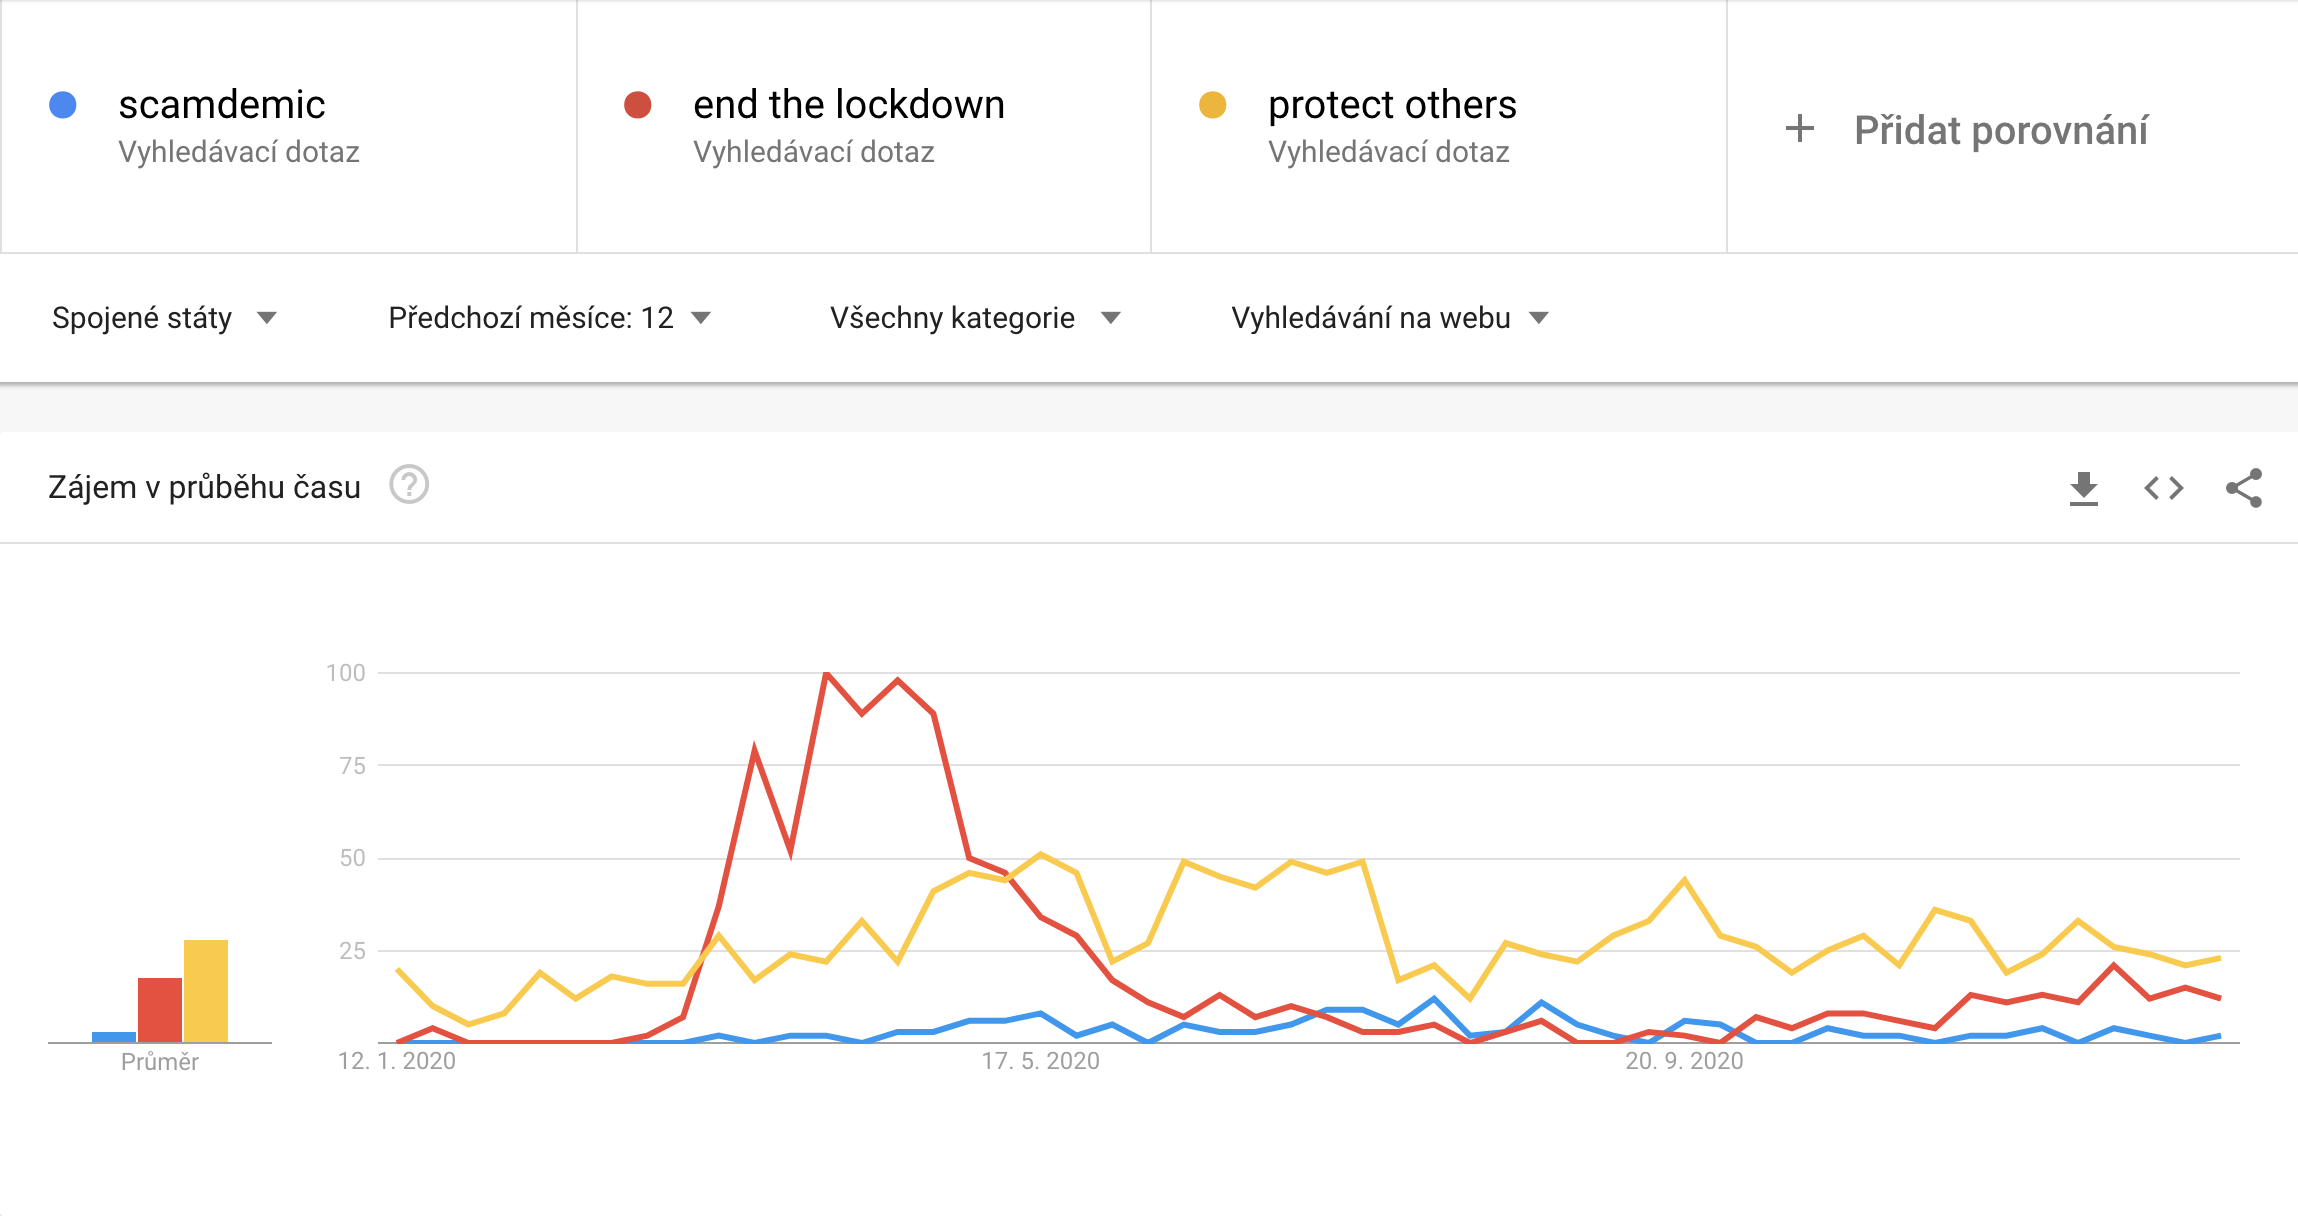
\includegraphics[width=14cm]{google_trends_analysis.png}
  \caption{Obrázek}
  \label{fig:google trends}
\end{figure}

Je možné pozorovat, že přes fakt, že pozitivní výraz \textit{protect the others} má v celém časovém období větší medián počtu vyhledávání, na začátku pandemie ho heslo \textit{end the lockdown} v počtu vyhledávání hravě předčilo, přičemž v poslední části grafu na něj nebezpečně znovu dotahuje, odhaduji, že především kvůli nechuti lidí řídit se dále vládními nařízeními a doporučeními kvůli délce trvání pandemie.\\

Při zadání samotného hesla do vyhledávače od Googlu můžeme dojít k následujícímu:\\

\begin{centering}
\begin{tabular}{l|c}
 \textbf{Vyhledávané heslo} & \textbf{Počet vyhledaných výsledků} \\ 
\hline
\hline
 \textit{scamdemic} & 1,270,000 results \\  
 \textit{end the lockdown} & 537,000,000 results \\
 \textit{protect others} & 1,420,000,000 results \\
\hline
\hline    
\end{tabular}
  \captionof{table}{Krásná tabulka}
  \label{tbl:odkaz}
\end{centering}
\vspace*{5mm}

Byl by nutný další reserch pro odfiltrování důvěryhodných informací ohledně dezinformací od dezinformací, pro získání odpovídajícího čísla, nicméně myslím si, že pro ilustraci, kolik takových příspěvků je, jaká je to pro ně živná půda, a kolik z nich potenciálně může být dezinformačních to stačí.\\

Rovněž je vidět korelace mezi počtem vyhledávání a množstvím výsledků, z čehož dovozuji, že si vytvářející dezinformace úmyslně vybírají více užívaná hesla, samozřejmě tento bod je k diskuzi, neboť samotná korelace neznamená kauzalitu.\\

\newpage

\section{Jak proti dezinformacím bojovat?}

Jak je zřejmé z výše uvedeného, dezinformace představují velkou hrozbu, jak se proti nim ale účinně bránit?\\

Již v úvodu, při definování pojmu dezinformace, jsem zmínil, že dezinformace jsou nejvíce šířeny přes internet, a to zejména přes sociální sítě (problém mohou představovat zejména nemoderované sociální sítě jako například \textbf{Parler}), proto je zásadní, aby se velkou měrou o snahu vymítit dezinformace zasadili technologické společnosti jako Facebook, Twitter či Google a Microsoft, v českém prostředí by se měl zasadit o boj proti dezinformacím například Seznam, zejména pak při indexování webových stránek ve svém vyhledávači (a to tím, že dezinformační weby by nebyly indexovány).\\

Pozitivní je fakt, že snaha o boj proti dezinformacím se v poslední době stala pro tyto technologické giganty prioritou, proto reagují na dezinformace propagováním autoritativního obsahu, sdílením důvěryhodných informací od důvěryhodných zdrojů (vládní a nadnárodní zdravotnické agentury a to jak obecně tak i se zaměřením na vyhledávání těchto témat, tedy například při vyhledávání informací o Covid-19) a větší manuální i automatizovanou kontrolu sdíleného obsahu spojeného s takzvaným \textit{tagováním} potenciálně dezinformačního obsahu společně s jeho mazáním a blokací zdrojů, ze kterých tyto informace pocházeli. Další bojová linie pak byla zavedena na úrovni snahy o zabránění automatického vytváření a šíření dezinformačního obsahu dávkově, tedy bez přičinění člověka primárně za pomoci botů, to vedlo, a dovoluji si tvrdit, že i v budoucnu bude vést k nutnosti reálné autorizace uživatelů platforem.\\

\begin{figure}[htbp]
  \centering
  
\includegraphics[width=14cm]{this_claim_is_disputed.png}
  \caption{Takto může například vypadat \textit{otagování} dezinformačního příspěvku}
  \label{fig:disputed_claim}
\end{figure}

Současná krize a koordinovanější přístup technologický společností vedl ke změně pravidel užívání jednotlivých platforem vztahujících se především k šíření nepravd a polopravd a potenciální možnosti toho, že toto sdílení může vyvolat mnoho škod a dá se tak, alespoň s malým oddechem, počítat s tím, že takto nastolený nový přístup budou technologické společnosti a i klasická média držet i do budoucna.\\

%\newpage

Zatímco moderování obsahu zřejmě škodlivého, a to zejména s ohledem na fyzickou újmu, tedy například propagace perorálního požívání čístících prostředků jako prostředku k léčbě Covidu-19 je poměrně jednoduchá a lze mnohakdy zachytit automatizovaným způsobem, řešení dezinformací při vznikající, respektive nově vzniklé/objevené pandemii je s ohledem na mnoho neznámých složité (o nově vzniklém viru nemusí být v jeho prvopočátcích mnoho informací). Je tak složitější odhalit přímé dezinformace, neboť i oficiální a důvěryhodné zprávy se ve svých prvopočátcích nemusí opírat o množství jiných důvěryhodných zdrojů, a to zejména pokud určitým aspektům nové nemoci vědci při jeho objevení ze začátku nerozumí, to se ostatně stalo i v případě momentálně probíhající pandemie koronaviru, otázka v oblasti veřejného zdraví může být dále značně zpolitizována a podléhat častým změnám. Koncept prvního bodu stanoveného \textbf{WHO} (viz první kapitola) je tak složitější naplnit, stejně tak jako je složitější určit, jaké příspěvky mohou svojí informační/dezinformační povahou způsobit společnosti újmu.\\

Je proto logické, že si mnoho lidí pokládá otázku \textit{"Jak tedy vlastně proti dezinformacím máme bojovat?"}. Je nutné vzít v potaz několik zásaních otázek, které jsou doplňující k pohledu \textbf{WHO} na dezinformace:\\

\begin{enumerate}
\item Jakým způsobem by společnost jako celek i jednotlivci měli reagovat na šíření dezinformací/misinformací v případech, kdy o tématice není v danou chvíli mnoho informací, vědecká shoda a výzkum, jaké informace by tedy měly být propagovány, a jaké naopak netolerovány?
\item Jakým způsobem by společnost jako celek i jednotlivci měli přistupovat k, a čelit, dezinformacím v různých podobách?
\item Jaké podoby by měli být prioritizovány, mělo by se s veškerými dezinformacemi zacházet stejně (otázky, pochybné důkazy, vizualizace - obrázky, videa), tedy všechny hodnotit jako kategorii přímých nepravdivých či zavádějících tvrzení na základě jejich vnímaného záměru, či jejich potenciálních důsledků spočívajících primárně v možnosti způsobit újmu?
\item Po zodpovězení předchozích 3 bodů (jakožto k rozšíření bodu prvního vyslovené v první kapitole ze strany \textbf{WHO}, jaká by měla být nejefektivnější strategie pro zmírnění dopadu dezinformací a jejich následného vymícení jak v online, tak i v offline prostoru? 
\end{enumerate}
\vspace*{5mm}

Po zodpovězení prvních 3 (1) otázky tedy nastává ta nejdůležitější otázka, jak proti dezinformacím bojovat?\\

Již na začátku této kapitoly jsem nastínil způsoby, které používají technologické společnosti pro boj s dezinformacemi v online prostoru,  např. odstranění, snížení viditelnosti, \textit{otagování}, zavedení možnosti nahlášení. Komplexní obrana namířená přesně proti nově vznikajícím dezinformačním hrozbám tak ve svém výsledku, vzhledem k výše vyřčenému, může být komplikovaná ve velkém měřítku nejen díky masivním komunitám a velké diverzifikovanosti příspěvků a hesel, ale i vzhledem k rychlosti šíření dezinformací (viz zdroj ohledně rychlosti šíření dezinformací) v reálném čase.\\

Všechno řešení ale nespočívá jen v technologické sféře, potřeba ověřovat si informace a kritické myšlení společně s co největší informovaností musí být rozvíjeno i na individuální úrovni, což je konečně to, co může přispět k vymícení dezinformací, zatímco editační snahy (zmíněné výše) v online a offline zdrojích mohou pomoci, nejsou samospásné, finální fronta proti dezinformacím musí být individuálně u každého člověka. V individuální sféře každého člověka je tak vždy potřeba posilovat především vzdělání, osvětu a kritické myšlení.\\

U lidí, kteří jsou dezinformacemi ovlivněni se však můžeme setkávat i s argumentem, že snaha bojovat proti dezinformací (Twitter například dezinformační příspěvky maže, nebo k nim připojuje vysvětlivky, viz Obrázek č.~\ref{fig:disputed_claim}) se ve své podstatě rovná cenzuře, a že všechny názory by se měly tolerovat. Je tak podstatné nalézt odpověď i na tuto problematiku, aby společnost tomuto názoru dokázala s dostatečnou precizností obstát.\\

\newpage

Troufám si tvrdit, že dobré vysvětlení, proč není možné boj proti dezinformacím považovat za cenzuru poskytu následující grafika Obrázek č.~\ref{fig:tolerance_paradox}:\\

\begin{figure}[htbp]
  \centering
  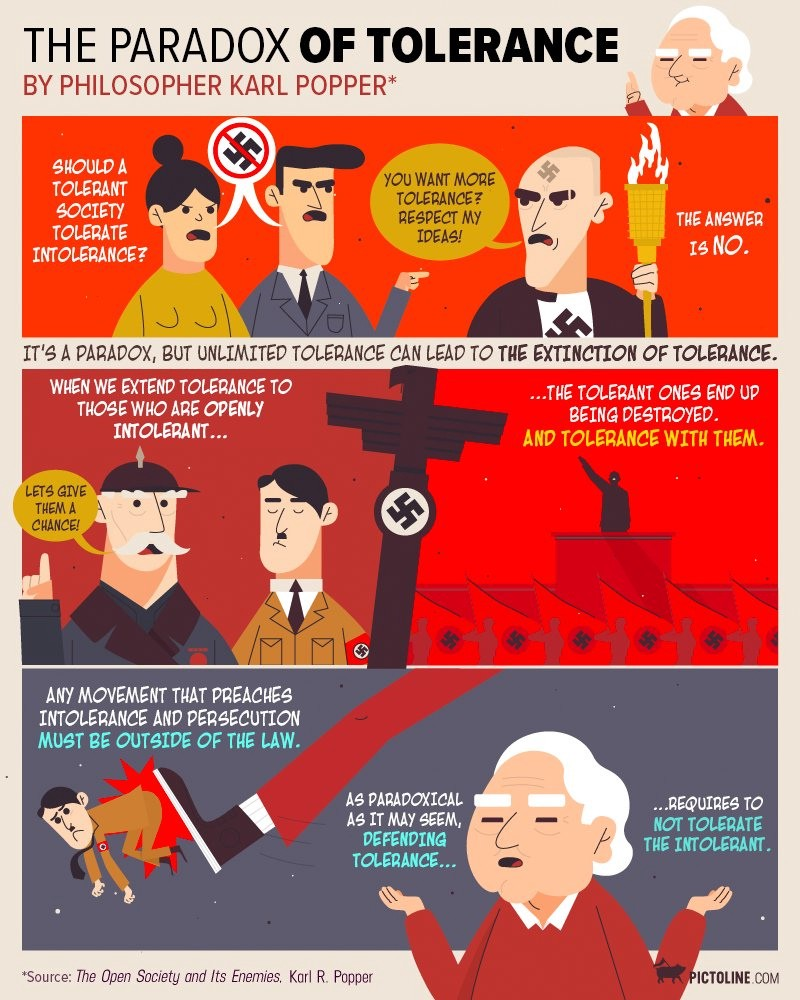
\includegraphics[width=12cm]{intolerance_vs_tolerance.jpeg}
  \caption{Paradox tolerance (zdroj)}
  \label{fig:tolerance_paradox}
\end{figure}

Diskuze o paradoxu tolerance je důležitá právě ve vztahu k dezinformacím, neboť ty jsou často chráněny pod heslem \textit{"svoboda projevu"}, zde se objevuje i tento jakýsi \textit{"informační paradox"}, neboť absolutní svoboda projevu stejně tak, jako absolutní tolerance, vede k potlačení toho, na čem stojí, tedy svobodě projevu.\\

\newpage

\section{Závěr}

Je zřejmé, že dezinformace představují velkou hrozbu pro moderní společnost, tato hrozba je v poslední době posílena i díky probíhající krizi, která zakládá živnou půdu pro jakékoliv dezinformační snahy.\\

S ohledem na nedávné události spojené například s volbami v USA můžeme vidět, kam až může šíření dezinformací zajít a k čemu může občany přimět.\\

Podobných dezinformačních snah si můžeme povšimnout i vzhledem k tématu světové pandemie, není tedy iluzurní myslet si, že jejich sdílení může vyůstit ve velice negativní následky. Ostatně dopad dezinformací je vidět v poslední době především k očkování, které je pro vyřešení krize klíčové. Cílová hodnota proočkování k překonání krize je 95\%(zdroj) obyvatelstva, dezinformace však mohou dosažení tohoto čísla značně ztížit a v konečném důsledku tak i v nejhorším možném případě zabránít, abychom se efektivně vypořádali s nákazou koronaviru. I nejen z toho důvodu je zásadní, abychom proti dezinformací ve všech oblastech důrazně vystupovali a bojovali za použití veškerých nám dostupných nástrojů.

